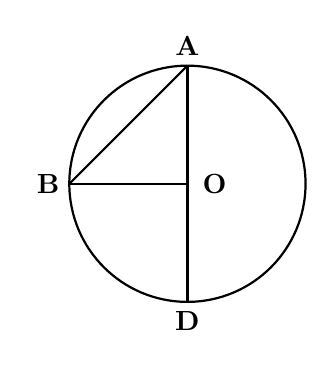
\begin{tikzpicture}[scale=1]

    % Define the center of the circle
    \coordinate (O) at (0,0);

    % Draw the circle with a radius of 1.5
    \draw[thick] (O) circle (1.5);

    % Define the coordinates for the points on the circle
    % A is at the top of the vertical diameter
    \coordinate (A) at (0, 1.5);
    % B is at the left of the horizontal radius
    \coordinate (B) at (-1.5, 0);
    % D is at the bottom of the vertical diameter
    \coordinate (D) at (0, -1.5);

    % Draw the vertical diameter AD
    \draw[thick] (A) -- (D);

    % Draw the horizontal radius OB
    \draw[thick] (O) -- (B);

    % Draw the chord AB connecting point A and point B
    \draw[thick] (A) -- (B);

    % Place the labels exactly as they appear in the image
    \node[above] at (A) {\textbf{A}};
    \node[left] at (B) {\textbf{B}};
    \node[right, xshift=2pt] at (O) {\textbf{O}};
    \node[below] at (D) {\textbf{D}};

\end{tikzpicture}